\section{\gls{ims} dataset No.2 - Bearing 1 sensor}
\label{sec:IMS_n2_3x}

In the previous sections, the framework capability for detecting novelties has been tested. Looking back to the \autoref{tab:IMS_test_parameters}, dataset No.2 shares the same type of fault as dataset No.3.

In order to further validate the \gls{nd}, in this section, a fresh training on dataset No.2 is performed. This time using the \gls{mla} for both performing the \gls{nd} and \gls{fd}.

\subsection{\gls{nd} instance}
The first instance of the \gls{mla} is used to detect the \gls{nd} event. The sensor declared in the configuration file is the one of Bearing 1, because it is the one that will experience outer race failure. The training is done on the first 300 snapshots of the dataset. The silhouette criterion suggested using 2 clusters. The \gls{mla} is then switched in evaluation mode, as usual. The novelty metric computed for the rest of the dataset is shown in \autoref{fig:IMS_n2_3x_nd}. 

The \gls{nd} event is triggered at 2004-02-16 03:32, 3~days before the end of the data acquisition. After the event, the novelty metric stays consistently over the threshold. 

\begin{figure}
    \centering
    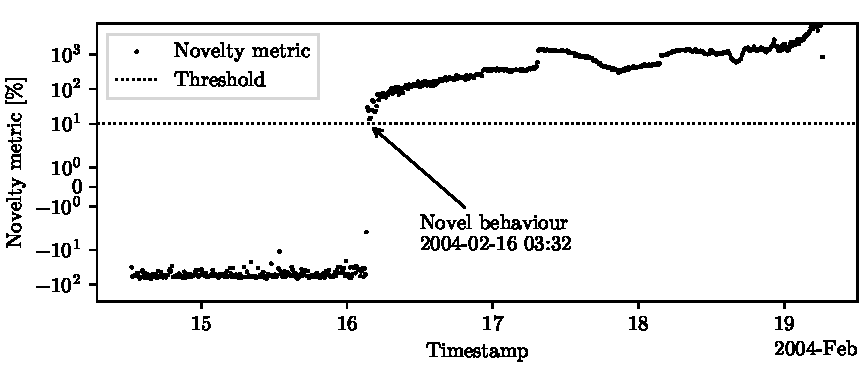
\includegraphics{images/IMS/Test02/ND.pdf}
    \caption{Novelty detection on the \gls{ims} dataset No.2 using the sensor of Bearing 1}
    \label{fig:IMS_n2_3x_nd}
\end{figure}

At this point, the \gls{rul} can be predicted at various instants after the \gls{nd} event. The \gls{rul} predictions are shown in \autoref{fig:IMS_n2_3x_prediction}. The predictions are made considering the last 250 snapshots of the dataset. Most predictions are accurate, except for the one done on 2004-02-18 03:32, which is affected by the temporary local decrease of the novelty metric. In this case, the last \gls{rul} estimation should be retained.

\begin{figure}
    \centering
    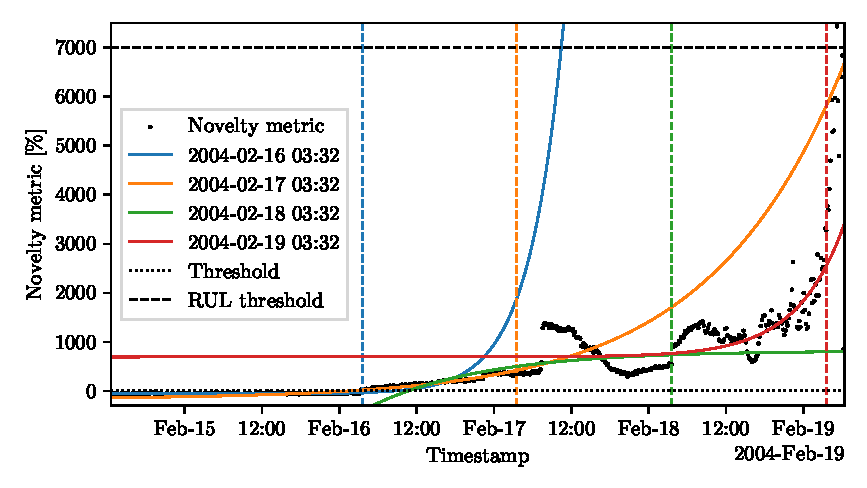
\includegraphics[width=\textwidth]{images/IMS/Test02/RUL.pdf}
    \caption{\gls{rul} prediction at different instants after the \gls{nd} event (dashed lines are the instants of the predictions corresponding to the same-colour solid line prediction)}
    \label{fig:IMS_n2_3x_prediction}
\end{figure}

\subsection{\gls{fd} instance}
The second instance of the \gls{mla} is used to detect the \gls{fd} event. The last 75 snapshots of the dataset are used for training. The silhouette criterion suggested using 8 clusters. The \gls{mla} is then switched in evaluation mode. 

In this case, the novelty metric provided by the \gls{mla} will be the transformed version, according to \autoref{eq:clust_eval_log}. In this case, a positive value of the metric corresponds to a known fault. When the metric becomes positive, the snapshot is already inside a faulty cluster, so the \gls{fd} event is triggered using a negative threshold. The novelty metric computed for the rest of the remaining samples in the dataset, after the set used to train the \emph{healthy} model and before the set used to train the \emph{faulty} model. The resulting metric is shown in \autoref{fig:IMS_n2_3x_fd}.

The \gls{fd} event is triggered at 2004-02-18 03:32, 1~day after the \gls{nd} event. After the event, the last 250 values of the novelty metric are used for \gls{rul} prediction. 

This example illustrates a scenario in which the \gls{nd} event is detected first, and then the \gls{fd} event confirms the presence of a known fault in the system.

\begin{figure}
    \centering
    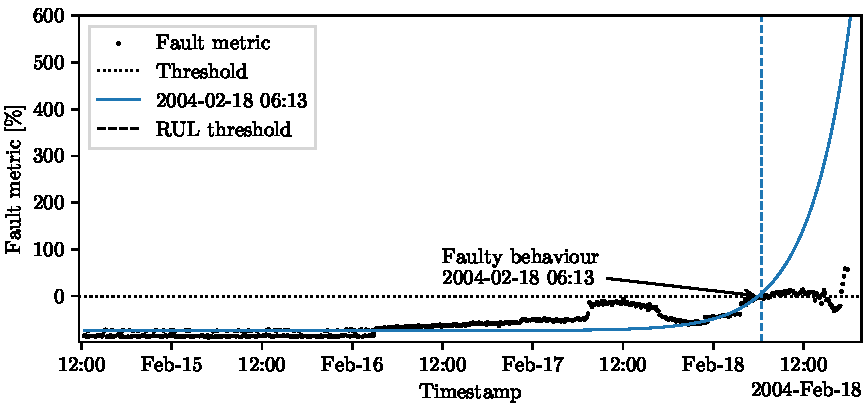
\includegraphics{images/IMS/Test02/FD.pdf}
    \caption{Fault detection on the \gls{ims} dataset No.2 using the sensor of Bearing~1}
    \label{fig:IMS_n2_3x_fd}
\end{figure}

